\documentclass[10pt,a4paper]{article}
\usepackage{tikz}
\usetikzlibrary{positioning}
\usetikzlibrary{matrix, arrows.meta}

\begin{document}
	
	\begin{figure}[h]
		\centering
		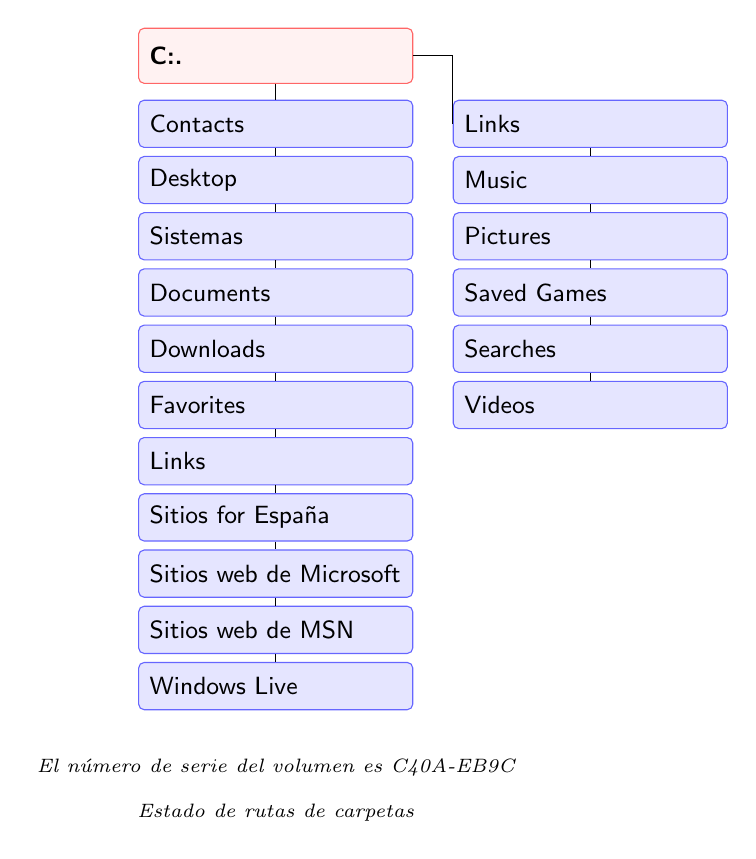
\begin{tikzpicture}[
			folder/.style={
				rectangle,
				minimum height=0.6cm,
				inner sep=4pt,
				text width=3.2cm,
				draw=blue!60,
				fill=blue!10,
				rounded corners=2pt,
				font=\small\sffamily,
				align=left
			},
			root/.style={
				rectangle,
				minimum height=0.7cm,
				inner sep=4pt,
				text width=3.2cm,
				draw=red!60,
				fill=red!5,
				rounded corners=2pt,
				font=\small\sffamily\bfseries,
				align=left
			}
			]
			% Raíz C:
			\node[root] (croot) {C:.};
			
			% Primera columna - Carpetas principales
			\node[folder, below=0.2cm of croot] (contacts) {Contacts};
			\node[folder, below=0.1cm of contacts] (desktop) {Desktop};
			\node[folder, below=0.1cm of desktop] (sistemas) {Sistemas};
			\node[folder, below=0.1cm of sistemas] (documents) {Documents};
			\node[folder, below=0.1cm of documents] (downloads) {Downloads};
			\node[folder, below=0.1cm of downloads] (favorites) {Favorites};
			\node[folder, below=0.1cm of favorites] (links) {Links};
			\node[folder, below=0.1cm of links] (sitiosespana) {Sitios for España};
			\node[folder, below=0.1cm of sitiosespana] (sitiosmicrosoft) {Sitios web de Microsoft};
			\node[folder, below=0.1cm of sitiosmicrosoft] (sitiosmsn) {Sitios web de MSN};
			\node[folder, below=0.1cm of sitiosmsn] (windowslive) {Windows Live};
			
			% Segunda columna - Carpetas adicionales (al mismo nivel)
			\node[folder, right=0.5cm of contacts] (links2) {Links};
			\node[folder, below=0.1cm of links2] (music) {Music};
			\node[folder, below=0.1cm of music] (pictures) {Pictures};
			\node[folder, below=0.1cm of pictures] (savedgames) {Saved Games};
			\node[folder, below=0.1cm of savedgames] (searches) {Searches};
			\node[folder, below=0.1cm of searches] (videos) {Videos};
			
			% Líneas conectivas desde la raíz
			\draw (croot.south) -- (contacts.north);
			\draw (contacts.south) -- (desktop.north);
			\draw (desktop.south) -- (sistemas.north);
			\draw (sistemas.south) -- (documents.north);
			\draw (documents.south) -- (downloads.north);
			\draw (downloads.south) -- (favorites.north);
			\draw (favorites.south) -- (links.north);
			\draw (links.south) -- (sitiosespana.north);
			\draw (sitiosespana.south) -- (sitiosmicrosoft.north);
			\draw (sitiosmicrosoft.south) -- (sitiosmsn.north);
			\draw (sitiosmsn.south) -- (windowslive.north);
			
			% Líneas para la segunda columna (conectadas también a la raíz)
			\draw (croot.east) -- ++(0.5,0) |- (links2.west);
			\draw (links2.south) -- (music.north);
			\draw (music.south) -- (pictures.north);
			\draw (pictures.south) -- (savedgames.north);
			\draw (savedgames.south) -- (searches.north);
			\draw (searches.south) -- (videos.north);
			
			% Información adicional (como en el comando tree)
			\node[below=0.5cm of windowslive, font=\scriptsize\itshape] (info1) {El número de serie del volumen es C40A-EB9C};
			\node[below=0.1cm of info1, font=\scriptsize\itshape] (info2) {Estado de rutas de carpetas};
			
		\end{tikzpicture}
		\caption{Estructura de carpetas de Windows - Comando \texttt{tree}}
		\label{fig:windows_tree_structure}
	\end{figure}
	
	\section{\textbf{Arrows}}
	
	\begin{figure}
		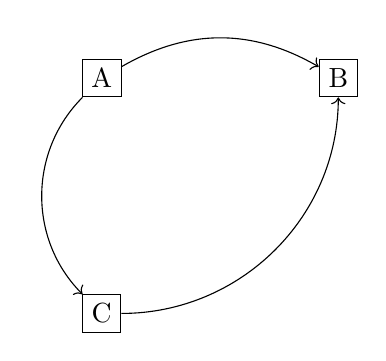
\begin{tikzpicture}[node distance=2.5cm]
			\node[draw] (A) {A};
			
			\node[draw, right=of A] (B) {B};
			\node[draw, below=of A] (C) {C};
			
			\draw[->, bend left=30] (A) to (B);        % curva suave
			\draw[->, bend right=45] (A) to (C);       % hacia abajo curvado
			\draw[->, out=0, in=270] (C) to (B);       % control manual
		\end{tikzpicture}
	\end{figure}
	
	
	
	\begin{figure}
		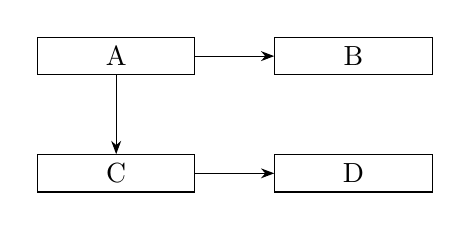
\begin{tikzpicture}[>=Stealth]
			\matrix[matrix of nodes, nodes={draw, minimum width=2cm}, row sep=10mm, column sep=10mm] (m) {
				A & B \\
				C & D \\
			};
			\draw[->] (m-1-1) -- (m-1-2);
			\draw[->] (m-1-1) -- (m-2-1);
			\draw[->] (m-2-1) -- (m-2-2);
		\end{tikzpicture}
	\end{figure}
	
	\section{Posiciones relativas}
	\begin{figure}
		\begin{tikzpicture}
			\draw[->] (0,0) -- ++(2,0);      % desde (0,0) hasta +2 en x
			\draw[->] (2,0) -- ++(0,2);      % desde el nuevo punto
		\end{tikzpicture}
	\end{figure}
	
	\section{Rutas Ortogonales}
	\begin{figure}
		\begin{tikzpicture}[node distance=2cm]
			\node[draw] (A) {A};
			\node[draw, below=of A] (B) {B};
			\node[draw, right=of B] (C) {C};
			
			\draw[->] (A) |- (B);   % baja y luego conecta
			\draw[->] (A) -| (C);   % primero derecha, luego baja
		\end{tikzpicture}
	\end{figure}
	
	\section{Conexion entre puntos}
	
	\begin{figure}
		\begin{tikzpicture}
			% Coordenadas sueltas
			\coordinate (A) at (0,0);
			\coordinate (B) at (3,-2);
			
			% Flecha ortogonal entre coordenadas personalizadas
			\draw[->, thick, teal] (A) |- (B);
			\draw[fill] (A) circle (2pt) node[above left]{A};
			\draw[fill] (B) circle (2pt) node[below right]{B};
		\end{tikzpicture}
	\end{figure}
	
	\end{document}